\documentclass [11pt]{articleSBPO}

\usepackage[brazil]{babel}
\usepackage[utf8]{inputenc}
\usepackage[T1]{fontenc}
\usepackage{graphics}
\usepackage[a4paper,top=3.3cm,left=2.9cm,right=2.9cm,bottom=2.5cm,noheadfoot]{geometry}
\usepackage{algorithm}
\usepackage{algorithmic}
\usepackage{times}
\usepackage{amsmath}
\usepackage{amssymb}
\usepackage{setspace}
\usepackage{graphicx}
\usepackage{subfig}
\usepackage{indentfirst}
\usepackage{icomma}
\usepackage{url}
\usepackage{longtable}
\usepackage{lscape}
\usepackage{array}
\usepackage[alf]{abntex2cite}
\usepackage{epstopdf}
\usepackage{rotating}
\usepackage{tikz}
\usetikzlibrary{arrows}
\newcommand{\up}[1]{\raisebox{1.3ex}[0pt]{#1}}
% \usepackage{latex8}
\floatname{algorithm}{Algoritmo}
\def\figurename{Figura}
\def\tablename{Tabela}


%     configurações do pacote algorithm
% \renewcommand{\algorithmcfname}{alg}
\floatname{algorithm}{Algoritmo}
\renewcommand{\algorithmicrequire}{\textbf{Entrada:}}
\renewcommand{\algorithmicensure}{\textbf{Saída:}}
\renewcommand{\algorithmicend}{\textbf{fim}}
\renewcommand{\algorithmicif}{\textbf{se}}
\renewcommand{\algorithmicthen}{\textbf{então}}
\renewcommand{\algorithmicelse}{\textbf{senão}}
\renewcommand{\algorithmicelsif}{\algorithmicelse\ \algorithmicif}
\renewcommand{\algorithmicendif}{\algorithmicend\ \algorithmicif}
\renewcommand{\algorithmicfor}{\textbf{para}}
% \renewcommand{\algorithmicto}{\textbf{até}}
\renewcommand{\algorithmicforall}{\textbf{para todo}}
\renewcommand{\algorithmicdo}{\textbf{faça}}
\renewcommand{\algorithmicendfor}{\algorithmicend\ \algorithmicfor}
\renewcommand{\algorithmicwhile}{\textbf{enquanto}}
\renewcommand{\algorithmicendwhile}{\algorithmicend\ \algorithmicwhile}
\renewcommand{\algorithmicloop}{\textbf{laço}}
\renewcommand{\algorithmicendloop}{\algorithmicend\ \algorithmicloop}
\renewcommand{\algorithmicrepeat}{\textbf{repita}}
\renewcommand{\algorithmicuntil}{\textbf{até que}}
\renewcommand{\algorithmicprint}{\textbf{imprima}}
\renewcommand{\algorithmicreturn}{\textbf{retorne}}
\renewcommand{\algorithmictrue}{\textbf{verdadeiro}}
\renewcommand{\algorithmicfalse}{\textbf{falso}}
\renewcommand{\algorithmicnot}{\textbf{não}}

%\usepackage{attrib}

%\usepackage{natbib} % pacote que traz o formato das citações por autor (não por números, que é o default do LaTeX)

\newtheorem{Lemma}{Lemma}
\newtheorem{Theorem}{Theorem}
\newtheorem{Condition}{Condition}

\def\nohyphen{\pretolerance=1000 \tolerance=1000 \hyphenpenalty=1000 \exhyphenpenalty=1000}

\setlength{\parindent}{1.50cm}












%%%%%%%%%%%%%%%%%%%%%%%%%%%%%%%%%%%%%%%%%%%%%%%%%%%%%%%%%%%%%%%%%%%%%%%%%%%%%%%%%%%%%%%%%%%%%%%%%%%%%%
%%											 ATUALIZAR												%%
\newcommand{\sigla}[0] {SIMPL }
\newcommand{\nome}[0] {Sistema Interativo para Métodos de Programação Linear}
%%%%%%%%%%%%%%%%%%%%%%%%%%%%%%%%%%%%%%%%%%%%%%%%%%%%%%%%%%%%%%%%%%%%%%%%%%%%%%%%%%%%%%%%%%%%%%%%%%%%%%

\begin{document}
\pagestyle{empty}%tira a numeração das páginas

\thispagestyle{empty}%tira a numeração da página em questão

\begin{center}
\LARGE{\textbf{\normalsize \sigla: uma ferramenta online para ensino de programação linear}}
\end{center}

\vspace{5mm}

%%%%%%%%%%%%%%%%%%%%%%%%%%%%%%%%%%%%%%%%%%%%%%%%%%%%%%%%%%%%%%%%%%%%%%%%%%%%%%%%%%%%%%%%%%%%%%%%%%%%%%
%%											 ATUALIZAR												%%
\begin{center}
\textbf{André F. R. Malta$^{\alpha}$, Daniel G. de Oliveira$^{\alpha}$, Elias L. da S. Júnior$^{\alpha}$, João M. M. da C. Cota$^{\alpha}$, André R. da Cruz$^{\beta}$} \\
Centro Federal de Educação Tecnológica de Minas Gerais (CEFET-MG)  Campus Timóteo, \\
Rua 19 de Novembro, 121 – Centro, Timóteo - MG, Brasil \\
\{andrmalta, eliasluizjr\}@gmail.com \\
\{daniel.gdo, joao\_marcos\_cota\}@hotmail.com.com \\
\par
$\alpha$ Graduando em Engenharia da Computação \\
$\beta$  \\ 
\end{center}
%%%%%%%%%%%%%%%%%%%%%%%%%%%%%%%%%%%%%%%%%%%%%%%%%%%%%%%%%%%%%%%%%%%%%%%%%%%%%%%%%%%%%%%%%%%%%%%%%%%%%%


\begin{center}
{\bf RESUMO}
\end{center}
\nohyphen{ 


\noindent \textbf{PALAVRAS CHAVE. } 

\vspace{11pt}

\noindent \textbf{Áreas Principais: }
}

\begin{center}
{\bf ABSTRACT}
\end{center}
\nohyphen{


\noindent \foreignlanguage{english}{\textbf{KEYWORDS. }}

\vspace{11pt}

\noindent \foreignlanguage{english}{\textbf{Main areas: }}
}

\newpage

\section{Introdução}\label{sec:introducao}
Após a Revolução Industrial, houve um contínuo crescimento de organizações pelo mundo, fazendo com que as pequenas oficinas de artesãos dessem lugar a grandes organizações com variados setores, o que agregou complexidade de produção de produtos. Devido a essa complexidade surgiu a Pesquisa Operacional (PO), que segundo \cite{hillier} é aplicada a problemas envolvendo como conduzir e coordenar as operações (isto é, as atividades) em uma organização. A PO abrange diversas áreas como manufatura, transportes, construção, telecomunicações, planejamento financeiro, entre outros. Para encontrar a melhor solução de um problema de otimização, também chamada solução ótima, um modelo matemático deve ser gerado mantendo as características e restrições do problema.

Para otimização de um problema em PO são utilizadas algumas métricas de cálculos para a sua solução. Tais métricas podem ser trabalhosas se executadas manualmente em problemas com muitas variáveis e restrições. Para tal problema, existem algumas ferramentas que resolvem tais problemas de PO, conhecidos como solvers. Alguns desses solvers são o Gurobi da Gurobi Optimization, Inc. \cite{gurobi}, o Lingo e Lindo da Lindo System, Inc. \cite{lindo}, o GLPK: GNU Linear Programming Kit  \cite{glpk} e o lp\_solve \cite{lpsolve}. Outro problema enfrentado em geral por estudantes, é a dificuldade de entender como funcionam os algoritmos usados em PO em um problema. Para isso, existem solvers de fins didáticos acompanhadas de livros de PO como o TORA \cite{taha}. 

Existem poucos solvers didáticos gratuitos disponíveis na web que apresentem a resolução detalhada de problemas de Programação Linear (PL) e Programação Linear Inteira (PLI). Grande parte desses solvers não possuem uma interface intuitiva para o usuário ou demandam muito tempo do usuário na inserção de valores de um determinado problema a cada vez que se tem acesso ao sistema.

Este trabalho apresenta o \sigla (\nome), que é um solver didático gratuito disponível na Internet, com o intuito de auxiliar estudantes na compreensão de problemas de PO, utilizando-se dos métodos Simplex, \textit{Branch and Bounch} e de alguns métodos de alocação de recurso, como o Canto Noroeste, Menor Custo e Aproximação de Vogel. Através dele, é possível inserir modelos matemáticos a serem solucionados e serem salvos em arquivo de texto. Também apresenta o detalhamento da resolução, visando facilitar o entendimento do usuário dos métodos aplicado ao modelo inserido. O \sigla foi desenvolvido utilizando as linguagens \textit{Javascript, CSS3 e HTML5} e o \textit{framework Bootstrap} para desenvolvimento da interface. A biblioteca \textit{glpk.js} foi utilizada para a resolução de alguns problemas inseridos.

O trabalho está organizado da seguinte forma: a seção \ref{sec:fundamentacao} apresenta uma definição breve e formal dos métodos presentes no solver para resolução de problemas de PL; a seção \ref{sec:desenvolvimento} explica de forma mais técnica como o sistema foi desenvolvido. Já na seção \ref{sec:resultados} é mostrado o funcionamento do sistema final. Por fim, na seção \ref{sec:conclusao} há as considerações finais e sugestões de trabalhos futuros.

\section{Fundamentação Teórica}\label{sec:fundamentacao}


\subsection{Simplex}\label{subsec:Simplex}

O método Simplex proposto por George Dantzig, é um método matricial para resolver problemas de Programação Linear. Ele executa iterativamente em busca da solução ótima entre as soluções básicas viáveis. 

Abaixo são apresentados os passos iterativos do método em busca da solução ótima.

\begin{enumerate}
	\item \textbf{Inicialização}: Configurar para iniciar iterações, inclusive encontrar uma solução ponto extremo viável.
	\item \textbf{Teste de Otimalidade}: A solução ponto extremo viável atual é ótima?
	\begin{itemize}
		\item \textit{Caso positivo}: Pare e retorne a solução.
		\item \textit{Caso negativo}: Continue a iteração.
	\end{itemize}
	\item \textbf{Iteração}: Encontre uma solução ponto extremo viável adjacente melhor que a atual e vá para o passo 2.
\end{enumerate}

\subsubsection{Método do Grade M}\label{subsubsec:grandem}

Em um problema de PL, se houverem restrições que demandem variáveis artificiais, elas são inseridas para formar uma solução inicial semelhante a um problema em que todas as variáveis são de folga. O Simplex Grande M consiste em aplicar grandes punições as variáveis artificiais na função objetivo, fazendo com que tenham valor 0 na solução ótima.
Porém, esses altos valores de M podem gerar grandes erros de arredondamento. 

\subsubsection{Método das Duas Fases}\label{subsubsec:duasfases}

O método Duas Fases elimina essa constante M e resolve o método através de duas fases:

\begin{enumerate}
	\item Tenta encontrar uma solução inicial básica. Se achar, passa para a fase 2.
	\item É chamada para resolver o problema original.
\end{enumerate}

\subsubsection{Método do Simplex Generalizado}\label{subsubsec:generalizado}

O Simplex generalizado é usado quando a solução básica inicial é não factível e não ótima. Portanto, quando a solução é infactível, usa-se as regras do Simplex dual até restabelecer a viabilidade ou certificar que não existe solução factível. Quando a solução é factível, basta aplicar as regras do Simplex primal.

\subsection{Branch and Bound}\label{subsec:bnb}

O Branch and Bound é uma técnica desenvolvida para resolver problemas de PLI utilizando o método Simplex. Cada iteração da técnica é composta por um problema de PL solucionado através do algoritmo Simplex. Essa iteração é um nó na árvore de soluções, e a partir do resultado obtido esse nó pode ou não se tornar raiz de uma subárvore de possíveis soluções.

O algoritmo é descrito a seguir:

\bigskip

\noindent O modelo no nó analisado é resolvido pelo Simplex. Verificamos se o valor da função objetivo $Z$ é melhor que o da solução ótima atual.
\begin{itemize}
	\item \textit{Caso positivo}: Verificamos o conjunto de variáveis $x$, testando se $\forall  x_{i} \in x, x_{i} \in \mathbb{Z}$.
	\begin{itemize}
		\item \textit{Caso positivo}: O nó atual passa a ser a nova solução ótima.
		\item \textit{Caso negativo}: O valor da função objetivo $Z$ é substituído por $-\infty$ em problemas de maximização e $\infty$ nos de minimização. Escolhe-se uma variável $x_{i} \in x | x_{i} \notin \mathbb{Z}$ e gere dois novos modelos, adicionando para um a restrição $x_{i}' \leq \lfloor x_{i} \rfloor$ e para o outro $x_{i}'' \geq \lceil x_{i} \rceil$.
	\end{itemize}
	\item \textit{Caso negativo}: A solução é descartada. 
\end{itemize}

\subsection{Algoritmos de Transporte}\label{subsec:transporte}

O problema de transporte é uma sub-classe de Programação Linear que trata do envio de mercadorias de uma origem a um destino, sendo executada através de uma rota ótima, ou seja, com menor custo, tempo e que satisfaça as restrições de fornecimento e demanda. Tal analogia pode ser abrangida para outras áreas que lidam com alocação de recursos, como controle de estoque, programação de empregos, entre outros.

Segundo \cite{taha}, O problema geral consiste em $m$ origens e $n$ destinos, cada um representado por um nó, conforme mostra a Figura \ref{fig:grafotransporte}. As arestas representam o trajeto entre origem e destino. Em cada um, são determinadas duas características:

\begin{itemize}
	\item O custo de transporte por unidade em um trajeto;
	\item A quantidade enviada.
\end{itemize}

\begin{figure}[!h]
	\centering
	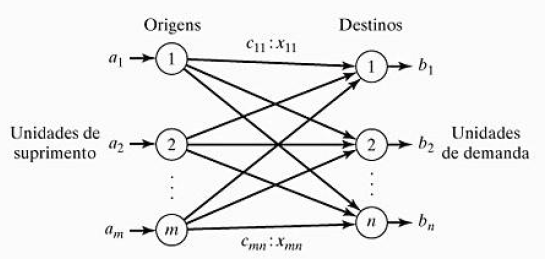
\includegraphics[width=0.5\textwidth]{img/grafotransporte.png}
	\caption[]{Grafo esquemático de um problema de transporte genérico}
	\label{fig:grafotransporte}
\end{figure}

\begin{table}[]
	\centering
	\caption[]{Representação em forma tabular de um problema de transporte genérico}
	\label{fig:tabelatransporte}
	\begin{tabular}{ l | l  l  l  l | l }
				& $b_{1}$ 	& $b_{2}$ 	& ... & $b_{n}$  & Suprimento\\
				\hline
	$a_{1}$		& $c_{11}$ 	& $c_{12}$	&  	  & $c_{1n}$ & $s_{1}$\\
	$a_{2}$		& $c_{21}$ 	& $c_{22}$	&  	  & $c_{2n}$ & $s_{2}$\\
	...			&  &  &  &  & \\
	$a_{m}$		& $c_{m1}$ 	& $c_{m1}$	&  	  & $c_{mn}$ & $s_{m}$\\
				\hline
	$Demanda$	& $d_{1}$ 	& $d_{2}$ 	& 	  & $d_{n}$	 & \\
	\end{tabular}
\end{table}

Sendo $a_{i}$ a origem de um trajeto, $b_{j}$ o destino, $c_{ij}$ o custo do trajeto, $x_{ij}$ a quantidade alocada para o trajeto, $s_{i}$ o suprimento máximo fornecido por $a_{i}$ e $d_{j}$ a demanda máximo de $b_{j}$

O objetivo do problema é determinar essa quantidade enviada ótima, de forma a satisfazer as restrições de demanda e suprimento.

Podemos determinar a quantidade enviada através de cada trajeto utilizando o método Simplex. Porém há outras técnicas mais rápidas e que garantem resultados próximos ao ótimo. Essas técnicas, apresentadas nos próximos tópicos, são preferidas para modelos muito grandes justamente pela sua simplicidade.

%\begin{tikzpicture}[->,>=stealth',shorten >=1pt,auto,node distance=3cm, thick,main node/.style={circle,draw,font=\sffamily\Large\bfseries}]
%
%\node[main node] (1) {$a_{1}$};
%\node[main node] (2) [below of=1] {$a_{2}$};
%\node[main node] (3) [below of=2] {$a_{m}$};
%\node[main node] (4) [right of=1] {$b_{1}$};
%\node[main node] (5) [below of=4] {$b_{2}$};
%\node[main node] (6) [below of=5] {$b_{n}$};
%
%\path[every node/.style={font=\sffamily\small}]
%(1) edge [left] {$c_{11} * x_{11}$} (4)
%	edge [left] (5)
%	edge [left] (6)
%(2) edge [left] (4)
%	edge [left] (5)
%	edge [left] (6)
%(3) edge [left] (4)
%	edge [left] (5)
%	edge [left] (6);
%\end{tikzpicture}

\subsubsection{Método do Canto Noroeste}\label{subsubsec:noroeste}

O mais simples dos métodos, porém o que pode apresentar pior resultado.

Seu princípio consiste em alocar recursos de acordo com a posição do trajeto na tabela de custos. Isso o torna altamente sensível à organização dos dados.

Segue o algoritmo abaixo:

\begin{enumerate}
	\item Inicia-se o algoritmo na primeira linha e primeira coluna.
	\item Aloca-se à célula atual o máximo de recursos permitidos pela oferta e demanda. \label{cantonoroeste:laco}
	\item Caso o suprimento da linha atual seja esgotado, desloca-se para a linha de baixo.
	\item Caso a demanda da coluna atual seja suprida, desloca-se para a coluna à direita.
	\item Se ainda houverem demandas a serem supridas retornar ao passo \ref{cantonoroeste:laco}.
\end{enumerate}

\subsubsection{Método do Menor Custo}\label{subsubsec:menorcusto}

O método do menor custo se concentra em rotas mais baratas. Com isso, seus resultados costumam ser melhores que o canto noroeste e não dependem de como o problema foi organizado na forma tabular.

Segue o algoritmo abaixo:

\begin{enumerate}
	\item Escolhe-se a célula com menor custo dentre as quais há demanda e oferta. \label{menorcusto:laco}
	\item Aloca-se à célula atual o máximo de recursos permitidos pela oferta e demanda. Resolva empates arbitrariamente.
	\item Caso ainda seja necessário alocar recursos, retornar ao passo \ref{menorcusto:laco}.
\end{enumerate}

\subsubsection{Método da Aproximação de Vogel}\label{subsubsec:mav}

Segundo \cite{taha}, o MAV é uma versão melhorada do método de menor custo e costuma produzir soluções melhores já que usa uma heurística mais complexa para determinar as melhores rotas.

Os passos seguidos pelo método são:

\begin{enumerate}
	\item Para cada linha e coluna determina-se uma multa subtraindo o menor custo do segundo menor custo. \label{mav:laco}
	\item Na linha ou coluna com maior multa escolha a célula com menor custo. Resolva empates arbitrariamente.
	\item Caso ainda não tenha completado o processo de alocação, retornar ao passo \ref{mav:laco}.
\end{enumerate}

%%%%%%%%%%%%%%%%%%%%%%%%%%%%%%%%%%%%%%%%%%%%%%%%%%%%%%%%%%%%%%%%%%%%%
%% CITACOES E REFERENCIAS

\section{Desenvolvimento}\label{sec:desenvolvimento}

O SIMPL é uma ferramenta desenvolvida com o intuito de fornecer o entendimento sistêmico do comportamento dos métodos de problemas de Programação Linear (PL) e Programação Linear Inteira (PLI). Para tal, a ferramenta possui uma didática de ensino, não focando em massivos dados de entrada. Portanto, é apropriada a todos os que desejarem ter maior conhecimento das técnicas e métodos utilizados para resolver variados problemas de Pesquisa Operacional e interagir com o sistema gerindo decisões a serem tomadas sobre os passos dos algoritmos.

Para mais fácil acesso, o trabalho desenvolvido em plataforma web e codificado utilizando-se a linguagem de programação \textit{JavaScript}, delegando os cálculos para a máquina cliente e reduzindo a carga na rede e nos servidores \cite{livrojavascript1}. Sendo então cada máquina responsável pelos próprios cálculos obtemos um melhor desempenho, processando os dados assim que o usuário necessita, sem perdas por latência de rede e sobrecargas no servidor. O \textit{CSS3 (Cascading Style Sheets versão 3)} é o elemento de definição de estilos para páginas Web, e foi utilizado no trabalho devido ao seu padrão ser adotado pela maioria dos navegadores disponíveis \cite{livroweb2}. O \textit{HTML (Hypertext Markup Language)} é uma linguagem para estruturação e apresentação de conteúdo em páginas WEB. A versão 5 do HTML foi utilizada, devido as suas novas funcionalidades como semântica, multimídia, interação e portabilidade, que são nativas da linguagem, sem a necessidade de uso de outras tecnologias \cite{livroweb1}.

Para a construção visual do trabalho realizado, utilizou-se do \textit{Bootstrap}, um \textit{framework} de desenvolvimento Web utilizando \textit{HTML, CSS} e \textit{JavaScript} para sistemas responsivos \cite{bootstrap}. Optou-se por sua utilização para exibição de elementos em tela que se adapta ao tamanho da tela de visualização. Para melhorar a interação do usuário com a interface fez-se uso da biblioteca \textit{jQuery}, que facilita a manipulação e acesso aos dados dos elementos \textit{HTML} e \textit{CSS} dinamicamente \cite{jquery}. Por fim, para a exibição de símbolos matemáticos nos modelos e resultados fez-se uso da biblioteca \textit{MathJax.js}, que permite a exibição de textos utilizando a linguagem \textit{TeX} em navegadores web \cite{mathjax}. Com o uso da linguagem \textit{TeX} é possível a descrição de símbolos em forma textual que são convertidos para sua respectiva representação gráfica, de forma que, quando necessário, possa ser feita a descrição através de notação matemática, trazendo mais clareza à comunicação entre programa e usuário \cite{tex}.

O \sigla até o momento da escrita desse artigo se divide em três partes: Simplex, \textit{Branch and Bound} e transporte. Cada uma dessas seções contém um formulário para entrada do modelo matemático e parametrização do método, opções para salvar e carregar modelos e páginas de ajuda informando mais sobre as técnicas e sobre como utilizar a ferramenta.

Os modelos criados podem ser utilizados para ver os resultados da execução completa do algoritmo ou cada iteração individualmente. Em ambos os casos são exibidas todas as etapas da execução dos algoritmos destacando as informações mais importantes que determinaram o curso tomado pelo algoritmo. É possível também fazer com que o algoritmo siga um caminho diferente caso o usuário deseje avaliar o que aconteceria de diferente. Essa alteração no caminho se dá de forma particular a cada método: no Simplex escolhe-se qual o elemento pivô, a partir do qual é definido qual variável sai e qual entra; no \textit{Branch and Bound} escolhe-se em qual variável não inteira será feito o processo de \textit{branching}, ou seja, adição de restrições ao valor daquela variável que cria dois modelos distintos; nos problemas de alocação de recursos, também chamados de problemas de transporte, o usuário pode escolher uma rota para ter recursos alocados.

Para que o método \textit{Branch and Bound} se mantivesse didaticamente intuitivo, foi construído uma árvore de representação de seus ramos. Para a construção dessa utilizou-se biblioteca \textit{vis.js}, permitindo a construção e manipulação de elementos gráficos em forma de árvore \cite{vis}. Além disso, como vários modelos Simplex devem ser executado nesse método, optou-se por utilizar uma biblioteca mais otimizada e que portanto possui melhor desempenho em vez do mesmo código criado para mostrar todas as iterações do Simplex. Para isso escolhemos o pacote \textit{GLPK (GNU Linear Programming Kit)} implementado na biblioteca \textit{glpk.js}. Apesar de a linguagem \textit{GNU MathProg} interpretada pelo \textit{GLPK} possuir diversos recursos, inclusive para PLI \cite{mathprog}, optou-se por realizar apenas o método Simplex de forma básica para que pudesse ser melhor exibido o processo de solução de diversos modelos de PL a fim de encontrar uma solução inteira.

\section{Resultados}\label{sec:resultados}



Para demonstrar o algoritmo Simplex foi utilizado o modelo abaixo, retirado de \cite{taha}, utilizando o Simplex Generalizado.

\begin{equation*}
	\begin{split}
		Minimizar\ z =\ & 4x_{1} + x_{2} \\
		sujeito\ a:\ \ \ \ &  3x_{1} + x_{2} = 3 \\
		& 4x_{1} + 3x_{2} \geq 6 \\
		& x_{1} + 2x_{2} \leq 4 \\
		& x_{1}, x_{2} \geq 0
	\end{split}
\end{equation*}

Na Figura \ref{fig:simplexit1} podemos observar o resultado exibido para a primeira iteração do algoritmo e como é mostrado para o usuário.

\begin{figure}[!h]
	\centering
	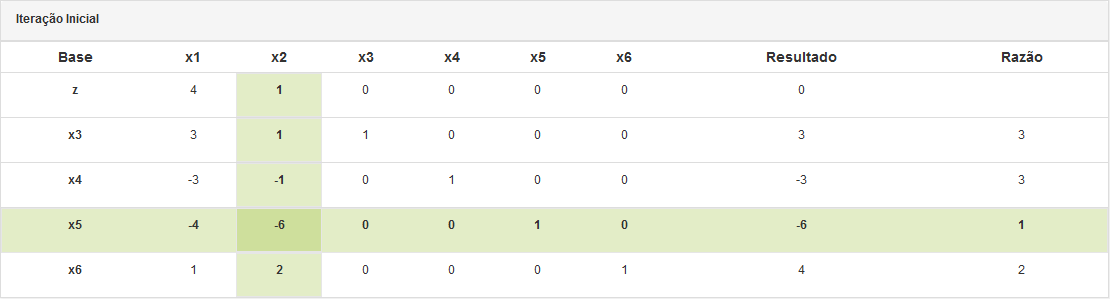
\includegraphics[width=0.9\textwidth]{img/simplexit1.png}
	\caption[]{Primeira iteração do algoritmo Simplex Generalizado}
	\label{fig:simplexit1}
\end{figure}

Observando a forma tabular do Simplex podemos notar que a iteração inicial está em uma solução inviável. Portanto o Simplex Generalizado usará técnicas do Simplex Dual para procurar uma nova solução, escolhendo nesse caso a variável de sobra $x_{5}$ para sair da base, inserindo a variável $x_{2}$ em seu lugar.

Após outras duas iterações, exibidas em forma simultânea e sequencial pela página, vemos a última iteração como demonstrado na Figura \ref{fig:simplexit3}. Como o estado atual de execução cumpre tanto a condição de viabilidade quanto de otimalidade o algoritmo termina sua execução. Com isso então, temos a solução ótima $x_{1}=0,4$ e $x_{2}=1,8$ com valor de função objetivo $z = 3,4$.

\begin{figure}[!h]
	\centering
	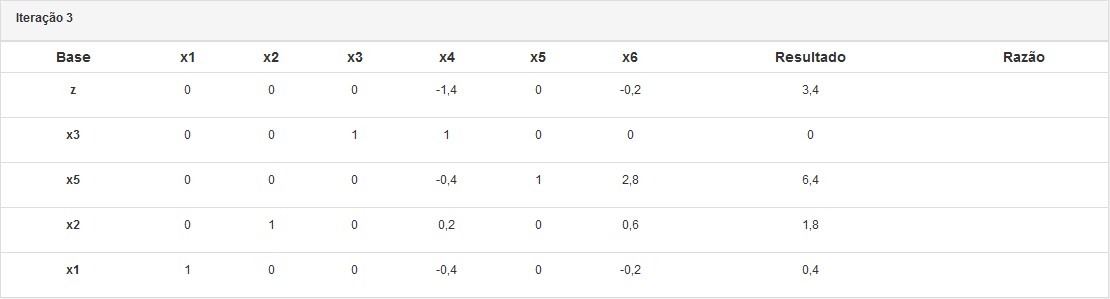
\includegraphics[width=0.9\textwidth]{img/simplexit3.png}
	\caption[]{Resultado final da execução do algoritmo Simplex}
	\label{fig:simplexit3}
\end{figure}

Já para demonstrarmos a execução do algoritmo \textit{Branch and Bound} será utilizado o modelo baixo, retirado de \cite{hillier}.

\begin{equation*}
\begin{split}
Maximizar\ z =\ & x_{1} + 5x_{2} \\
sujeito\ a:\ \ \ \ &  x_{1} + 10x_{2} \leq 20 \\
& x_{1} \leq 2 \\
& x_{1}, x_{2} \geq 0
\end{split}
\end{equation*}

Na Figura \ref{fig:bbno1} vemos o nó raiz da árvore de execução do algoritmo, que corresponde ao modelo inicial dado. Nesse caso a solução não é inteira, já que $x_{2}=1,8$ como destacado na parte inferior direita da imagem. Assim, o algoritmo cria dois novos nós: um adicionando uma restrição $x_{2} \leq 1$ e outro $x_{2} \geq 2$, sendo estes os nós 2 e 3 respectivamente.

\begin{figure}[!h]
	\centering
	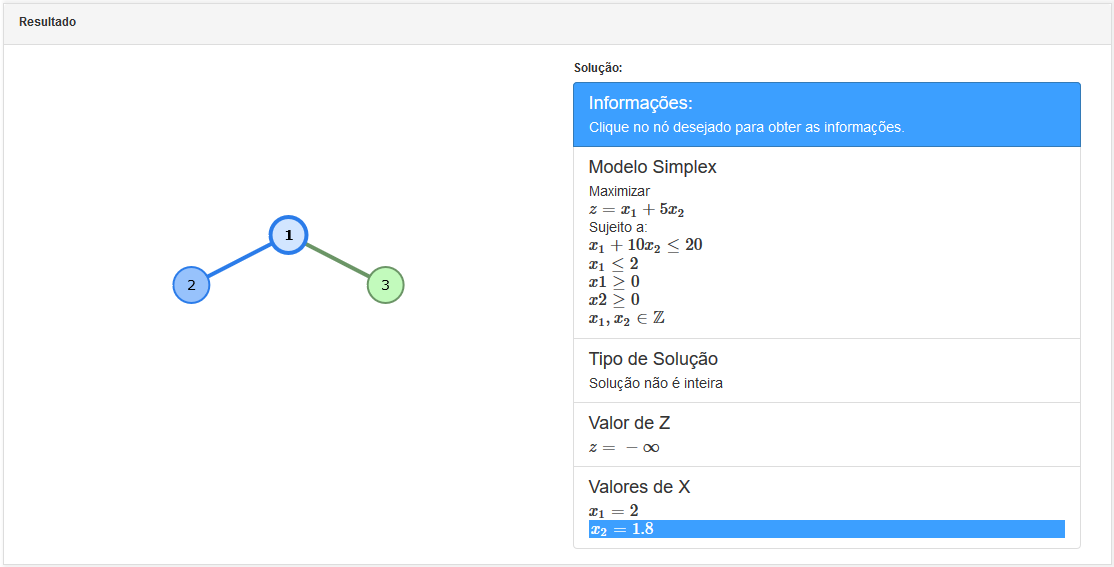
\includegraphics[width=0.8\textwidth]{img/bbno1.png}
	\caption[]{Nó raiz da árvore de execução}
	\label{fig:bbno1}
\end{figure}

O nó 2 teve solução $x_{1}=2$ e $x_{2}=1$ com valor de função objetivo $z = 7$ enquanto o nó 3 teve solução $x_{1}=0$ e $x_{2}=2$ com valor de função objetivo $z = 10$. Assim, como o nó 2 possui valor de $z$ pior que o do nó 3, este é considerado a solução ótima. Mesmo que a solução do nó 2 não fosse inteira, não haveria necessidade de continuar a execução nessa subárvore já que a solução não poderia ser melhor que a do nó 2, ocorrendo então o \textit{pruning}. O nó ótimo é destacado de verde, enquanto os nós sem solução viável destacados de vermelho. Para ver informações básicas sobre um determinado nó basta passar o mouse sobre o nó, como pode ser visto no nó 2, enquanto se clica sobre o nó para mostrar as informações de forma mais detalhada no painel à direita.

\begin{figure}[!h]
	\centering
	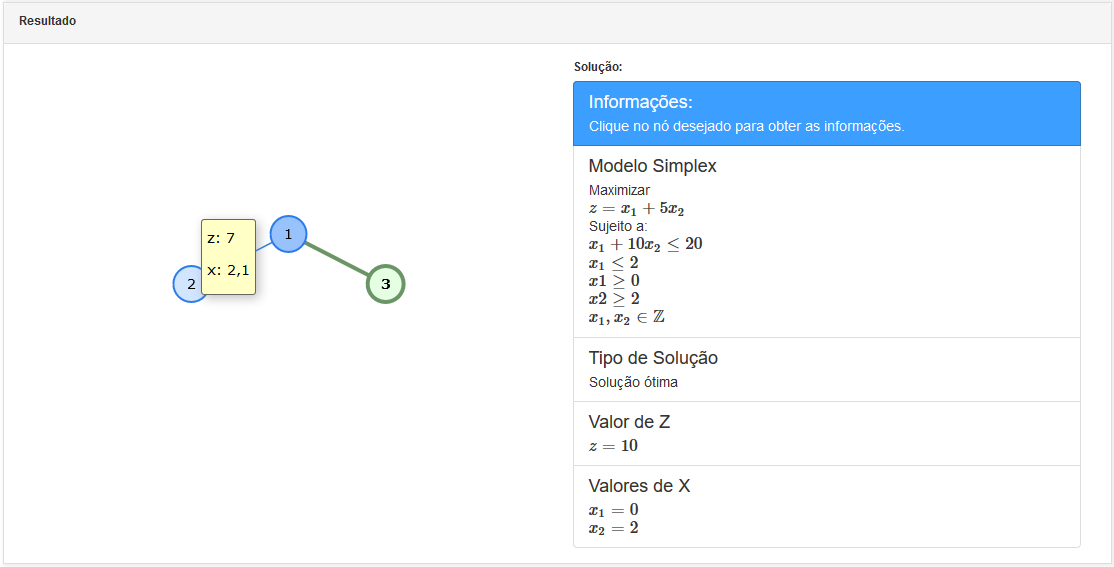
\includegraphics[width=0.8\textwidth]{img/bbno3.png}
	\caption[]{Nó ótimo da árvore de execução}
	\label{fig:bbno3}
\end{figure}

\section{Conclusões}\label{sec:conclusao}

\newpage

\bibliographystyle{abnt-alf}
\bibliography{referencias}

\end{document}